% Prijs van schoenen i.f.v. aantal
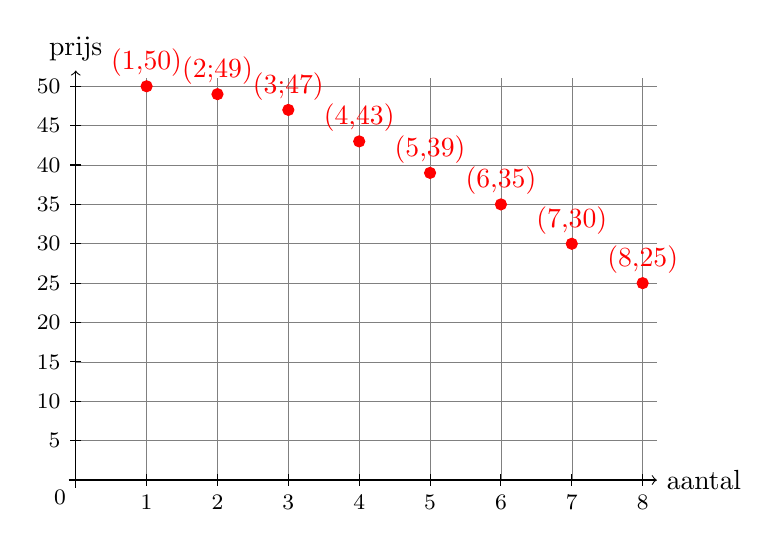
\begin{tikzpicture}[x=0.9cm,y=0.1cm]
\draw[help lines] (0,0) grid [xstep=1, ystep=5] (8.2,51);
\draw[->] (-0.1,0) -- (8.2,0) node[right] {aantal};
\draw[->] (0,-1) -- (0,52) node[above] {prijs};
\foreach \x in {1,...,8}
	\draw[shift={(\x,0)}] (0pt,2pt) -- (0pt,-2pt) node[below] {\footnotesize $\x$};
\foreach \y in {5,10,...,50}
	\draw[shift={(0,\y)},color=black] (2pt,0pt) -- (-2pt,0pt) node[left] {\footnotesize $\y$};
\node [below left] at (0,0) {\footnotesize 0};
\filldraw [red] (1,50) circle (2pt) node[above] {(1,50)};
\filldraw [red] (2,49) circle (2pt) node[above] {(2;49)};
\filldraw [red] (3,47) circle (2pt) node[above] {(3;47)};
\filldraw [red] (4,43) circle (2pt) node[above] {(4,43)};
\filldraw [red] (5,39) circle (2pt) node[above] {(5,39)};
\filldraw [red] (6,35) circle (2pt) node[above] {(6,35)};
\filldraw [red] (7,30) circle (2pt) node[above] {(7,30)};
\filldraw [red] (8,25) circle (2pt) node[above] {(8,25)};
\end{tikzpicture}